\chapter{State of the art}
\minitoc
\newpage

\setcounter{secnumdepth}{0} % Set the section counter to 0 so next section is not counted in toc
% ----------------------- Introduction ----------------------- %
\section{Introduction}
This chapter will present and study various concepts such as browser automation, web scraping, version control and DevOps with an emphasis on key DevOps terminologies.
We will talk about the most used tools in the market as well as which ones we settled on after making a comparison.

\setcounter{secnumdepth}{2} % Resume counting the sections for the toc with a depth of 2 (Sections and sub-sections)
% ----------------------- DevOps ----------------------- %
\section{Automation and Web Scraping concepts}
\subsection{Automation}
At its core, automation is leaving menial and recurring tasks to the automaton (or machine) in order to do more meaningful work as a human in the meantime.
Implementing automation improves the efficiency, reliability and the speed of tasks that previously took humans a lot of time.

\subsection{Web Scraping}
Web scraping is the process of automatically extracting content and data from a website.
Although data extraction is done in a brute way by reading texts from HTML elements, it is used in a variety of legitimate digital businesses like search engines, price comparison sites and market research companies.
So contrary to what some might think, web scraping is completely legal.

\subsection{Relationship between the two}
Web scraping simplifies the process of extracting data and the automation process helps repeating the recurring task of extraction.
As a result, the combination of scraping data, storing it and automating the whole process is getting very popular, especially with new technologies and tools arising in order to do just that.

% ----------------------- DevOps ----------------------- %
\section{DevOps}

\subsection{Definition}
DevOps is the set of practices, techniques and tools used to speed up the Software Development Lifecycle (SDL) by bringing together two historically separate functions of development and operations.

Development refers to writing code and software, whereas operations refer to provisioning servers, configuring them as well as deploying the apps to them, amongst other things.

DevOps teams focus on automating all of the above.
The key terminologies around DevOps are Continuous Integration, Continuous Delivery and Infrastructure As Code and automation.

\subsection{Lifecycle}
\begin{figure}[H]
    \centering
    \makebox[\textwidth]{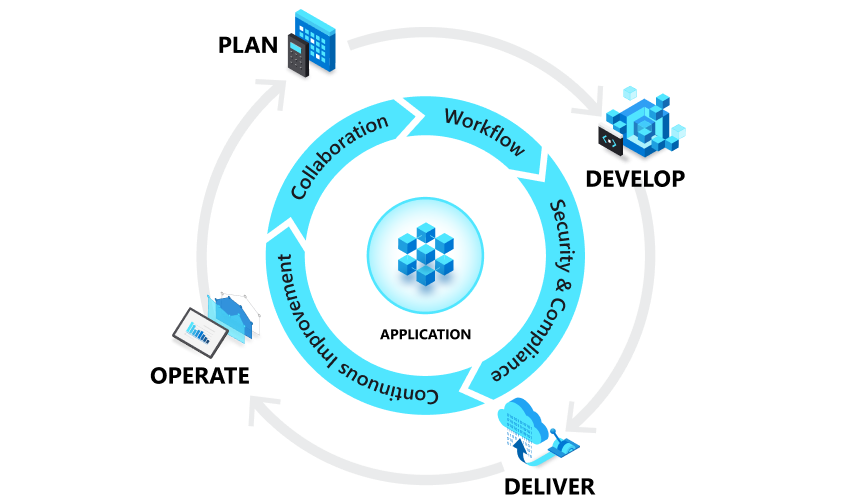
\includegraphics[width=12cm]{src/assets/images/devops-lifecycle.png}}
    \caption{DevOps and the application lifecycle}
    \label{fig:devops-lifecycle}
\end{figure}

DevOps -according to Microsoft Azure- is the main influencer of the application lifecycle throughout its plan, develop, deliver, and operate phases. All of the phases rely on one another and they are not role-specific. In a true DevOps culture, each role is involved in each phase to some extent. \cite{devops}

\begin{itemize}
    \item \textbf{Plan:} In this first stage, DevOps teams define and describe the main features of the system being created. They accomplish that by many ways. Some of which are creating backlogs, tracking bugs, using Kanban boards and visualizing progress with dashboards.
    \item \textbf{Develop:} This step includes all aspects of coding, testing, reviewing and code integration. It also includes creating build artifacts that can be deployed into various environments. Automation of mundane and manual tasks plays a heavy role in this phase through automated testing and continuous integration.
    \item \textbf{Deliver:} This is the process of deploying application into various environments such as staging or production consistently and reliably. It also includes deploying and configuring the infrastructure that makes up the environments. The DevOps team defines a release management process with automated gates or checkpoints the move the applications between stages in order to deploy in an efficient, scalable, repeatable and controllable way.
    \item \textbf{Operate:} The operate phase involves maintaining, monitoring and troubleshooting the application in the production environment. The purpose of this phase is ensuring high availability, system reliability and zero downtime. This requires alerting and full visibility into the application.
\end{itemize}

\subsection{Container management}
Containers have become an integral part of DevOps over the past couple of years but what are containers exactly and how do we manage them?

\subsubsection*{What is a container ?}
Simply said; container is a packaging format for software applications that are akin to a very lightweight virtual machine (very broad analogy) which always executes in an isolated environment \cite{what-is-a-container}.
What this implies is that said containers can be easily copied to and run on different machines with high reliability, lower costs and high efficiency.

\subsubsection*{What is container management ?}
Container management is the process for automating the creation, deployment and scaling of containers \cite{container-management}.
Container management tools such as Docker and Podman facilitate the addition, replacement and organization of containers.

\subsection{CI/CD pipelines}
A continuous integration and continuous deployment (CI/CD) pipeline is a series of steps that must be performed in order to deliver a new version of software.
CI/CD pipelines are a practice focused on improving software delivery throughout the software development life cycle via automation. \cite{cicd-definition}

% ----------------------- Microservices ----------------------- %
\section{Microservices}

\subsection{Definition}
Microservices are an architectural and organizational approach to software development where software is composed of small independent services that communicate over well-defined APIs.
These services are owned by small, self-contained teams. \cite{microservices}

\medskip
Microservices architectures make applications easier to scale and faster to develop, enabling innovation and accelerating time-to-market for new features.
\begin{figure}[H]
    \centering
    \makebox[\textwidth]{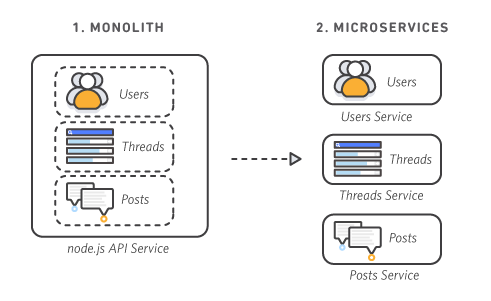
\includegraphics[width=12cm]{src/assets/images/microservices.png}}
    \caption{Monolith to microservices example}
    \label{fig:monolith-to-microservices}
\end{figure}
\subsection{Characteristics of Microservices}
\begin{itemize}
    \item \textbf{Autonomous:} Each component service in a microservices architecture can be developed, deployed, operated, and scaled without affecting the functioning of other services. Services do not need to share any of their code or implementation with other services. Any communication between individual components happens via well-defined APIs.
    \item \textbf{Specialized:} Each service is designed for a set of capabilities and focuses on solving a specific problem. If developers contribute more code to a service over time and the service becomes complex, it can be broken into smaller services.
\end{itemize}

\subsection{Benefits of Microservices}
\begin{itemize}
    \item \textbf{Agility:} Microservices foster an organization of small, independent teams that take ownership of their services. Teams act within a small and well understood context, and are empowered to work more independently and more quickly.
    \item \textbf{Flexible Scaling:} Microservices allow each service to be independently scaled to meet demand for the application feature it supports. This enables teams to right-size infrastructure needs, accurately measure the cost of a feature, and maintain availability if a service experiences a spike in demand.
    \item \textbf{Easy Deployment:} Microservices enable continuous integration and continuous delivery, making it easy to try out new ideas and to roll back if something doesn’t work. The low cost of failure enables experimentation, makes it easier to update code, and accelerates time-to-market for new features.
    \item \textbf{Technical Freedom:} Microservices architectures don’t follow a “one size fits all” approach. Teams have the freedom to choose the best tool to solve their specific problems. As a consequence, teams building microservices can choose the best tool for each job.
    \item \textbf{Reusable Code:} Dividing software into small, well-defined modules enables teams to use functions for multiple purposes. A service written for a certain function can be used as a building block for another feature. This allows an application to bootstrap off itself, as developers can create new capabilities without writing code from scratch.
    \item \textbf{Resilience:} Service independence increases an application’s resistance to failure. In a monolithic architecture, if a single component fails, it can cause the entire application to fail. With microservices, applications handle total service failure by degrading functionality and not crashing the entire application.
\end{itemize}

% ----------------------- Comparative Analysis ----------------------- %
\section{Comparative Analysis}
In order to get started with our project, we need a wide range of tools that deal with the following areas; version control, orchestration between containers, browser automation as well as scheduled automation. For that, we did a comparative study on some of the tools the market provides.

\subsection{Version Control: Git vs SVN}
The most used tools for version control are Git and SVN. Here is a table comparing both tools.
\begin{table}[H]
    \renewcommand{\arraystretch}{1.5}%
    \caption{Comparative study between Git and SVN}
    \centering
    \medskip
    \begin{tabularx}{1\textwidth} {
            | >{\hsize=.5\hsize\linewidth=\hsize\centering\arraybackslash}X
            | >{\hsize=1.25\hsize\linewidth=\hsize\justifying\arraybackslash}X
            | >{\hsize=1.25\hsize\linewidth=\hsize\justifying\arraybackslash}X |}
        \hline
        \rowcolor{primary} & \textbf {Description}                                                                                                                                   & \textbf {Advantages}                                                                                                                                                                     \\
        \hline
        \textbf{Git}       & \noindent Git is a distributed version control system which means that when cloning a repository, you get a copy of the entire history of that project. & \noindent Git has what's called a staging area. This means that even if you made over a 100 changes, they can be broken down to 10 commits each with their own comments and description. \\
        \hline
        \textbf{SVN}       & \noindent SVN or Subversion is a centralized version control system. Meaning that there is always a single version of the repository that you checkout. & \noindent SVN has one central repository – which makes it easier for managers to have more of a top down approach to control, security, permissions, mirrors, and dumps.                 \\
        \hline
    \end{tabularx}
\end{table}
In the end, both are great options. However, we will be using Git since the company already has a self-hosted GitLab instance that naturally uses Git.

\subsection{Container management: Docker vs Podman}
Although Docker is widely popular, Podman is also taking its share from the market. Especially on Red Hat systems.
\begin{table}[H]
    \renewcommand{\arraystretch}{1.5}%
    \caption{Comparative study between Docker and Podman}
    \centering
    \medskip
    \begin{tabularx}{1\textwidth} {
            | >{\hsize=.7\hsize\linewidth=\hsize\centering\arraybackslash}X
            | >{\hsize=1.15\hsize\linewidth=\hsize\justifying\arraybackslash}X
            | >{\hsize=1.15\hsize\linewidth=\hsize\justifying\arraybackslash}X |}
        \hline
        \rowcolor{primary} \textbf {Aspect} & \textbf {Docker}                                                                                                                                                                                                                    & \textbf {Podman}                                                                                                                                                                      \\
        \hline
        \textbf {Definition}                & \multicolumn{2}{|>{\hsize=2.35\hsize}X|} {Docker and Podman are both  container management technologies used to build container images and store said images in a registry to then run them as containers in a target environment.}                                                                                                                                                                                         \\
        \hline
        \textbf {Technology}                & \noindent Docker uses the containerd daemon which does the pulling of images then hands over the creation process to a low-level runtime named runc.                                                                                & \noindent Podman uses a daemon-less approach using a technology named conmon which does the heavy lifting. It also delegates the container creation to a low-level container runtime. \\
        \hline
        \textbf {Specificity}               & \noindent Docker Desktop is a great feature for Docker which provides an easy way to build and distribute containers amongst developers.                                                                                            & \noindent The smallest unit in Podman is the pod. A pod is the organizational unit for containers and is directly compatible with Kubernetes.                                         \\
        \hline
    \end{tabularx}
\end{table}
We can see the similarities between the two and in theory, it shouldn't really matter which one we choose since both Docker and Podman are inter-changeable.

\subsection{Browser automation: Puppeteer vs Playwright}
Both are Node.js libraries for browser automation. The table below compares these two on different levels.
\begin{table}[H]
    \renewcommand{\arraystretch}{1.5}%
    \caption{Puppeteer vs Playwright highlights}
    \centering
    \medskip
    \begin{tabularx}{1\textwidth} {
            | >{\hsize=.7\hsize\linewidth=\hsize\raggedright\arraybackslash}X
            | >{\hsize=1.15\hsize\linewidth=\hsize\justifying\arraybackslash}X
            | >{\hsize=1.15\hsize\linewidth=\hsize\justifying\arraybackslash}X |}
        \hline
        \rowcolor{primary} \textbf {Category} & \textbf {Puppeteer}                                                                                                                      & \textbf {Playwright}                                                                                                                                                         \\
        \hline
        \textbf {Overview}                    & \noindent Puppeteer makes it easy to get started with browser automation. This is in part because of how it interfaces with the browser. & \noindent Playwright is very similar to Puppeteer in many respects. The API methods are identical in most cases, and Playwright also bundles compatible browsers by default. \\
        \hline
        \textbf {Community}                   & \noindent Has a large community with lots of active projects.                                                                            & \noindent Small but active community.                                                                                                                                        \\
        \hline
    \end{tabularx}
\end{table}
Since the difference is pretty minor, we will be sticking to the more recent Playwright.

\subsection{Database: MongoDB vs PostgreSQL}
The old architecture of \glsxtrshort{ilg} uses PostgreSQL but we have the choice to use a different database as well, so we did the following study.
\begin{table}[H]
    \renewcommand{\arraystretch}{1.5}%
    \caption{Comparative study between MongoDB and PostgreSQL}
    \centering
    \medskip
    \begin{tabularx}{1\textwidth} {
            | >{\hsize=.7\hsize\linewidth=\hsize\centering\arraybackslash}X
            | >{\hsize=1.15\hsize\linewidth=\hsize\justifying\arraybackslash}X
            | >{\hsize=1.15\hsize\linewidth=\hsize\justifying\arraybackslash}X |}
        \hline
        \rowcolor{primary} \textbf {Category} & \textbf {MongoDB}                                                                 & \textbf {PostgreSQL}                                                                                         \\
        \hline
        \textbf {Overview}                    & \noindent An open-source NoSQL that stores data in JSON-like documents.           & \noindent An open-source relational database system.                                                         \\
        \hline
        \textbf {Storage}                     & \noindent Stores data in documents that belong to a particular class or group.    & \noindent Data is stored in tables where each table corresponds to an entity.                                \\
        \hline
        \textbf {Type}                        & \noindent NoSQL, meaning that data in a collection can have different structures. & \noindent Uses SQL (Standard Query Language) meaning that the schema of data cannot be changed once defined. \\
        \hline
    \end{tabularx}
\end{table}
Since the old architecture uses PostgreSQL, we will be sticking to that in the new architecture as well for an easier migration.

\subsection{Database: GraphQL vs REST}
One of the decision we need to make is how to exchange the data in our application.
For that, we compare GraphQL and REST.
\begin{table}[H]
    \renewcommand{\arraystretch}{1.5}%
    \caption{Comparative study between GraphQL and REST \cite{graphql-vs-rest}}
    \centering
    \medskip
    \begin{tabularx}{1\textwidth} {
            | >{\hsize=.6\hsize\linewidth=\hsize\centering\arraybackslash}X
            | >{\hsize=1.2\hsize\linewidth=\hsize\justifying\arraybackslash}X
            | >{\hsize=1.2\hsize\linewidth=\hsize\justifying\arraybackslash}X |}
        \hline
        \rowcolor{primary} & \textbf {Description}                                                                                                                          & \textbf {In depth}                                                                                                                          \\
        \hline
        \textbf{GraphQL}   & \noindent An open-source data query and manipulation language for APIs, and a runtime for fulfilling queries with existing data.               & \noindent Describe only what's needed in queries, so no under or over fetching. It is also Schema and Type safe so it's less prone to bugs. \\
        \hline\noindent
        \textbf{REST}      & \noindent REST (Representational State Transfer) is an architectural style that conforms to a set of constraints when developing web services. & \noindent It was introduced as a successor to SOAP APIs, follows the REST standards and is not constrained to XML.                          \\
        \hline
    \end{tabularx}
\end{table}
Due to time constraints, we agreed to use both.
GraphQL will be used internally between the microservices.
REST on the other hand will still be used by the frontend to communicate with the backend api service.

\subsection{Deployment: Docker Swarm vs Kubernetes}
The old deployment uses Docker Compose but that will not cut it anymore since it is not very optimized for production, especially on systems that need to scale later on as is the case here.
Our research leads us to choosing between either Docker Swarm or Kubernetes.

\begin{table}[H]
    \renewcommand{\arraystretch}{1.5}%
    \caption{Comparative study between Docker Swarm and Kubernetes}
    \centering
    \medskip
    \begin{tabularx}{1\textwidth} {
            | >{\hsize=.7\hsize\linewidth=\hsize\centering\arraybackslash}X
            | >{\hsize=1.15\hsize\linewidth=\hsize\justifying\arraybackslash}X
            | >{\hsize=1.15\hsize\linewidth=\hsize\justifying\arraybackslash}X |}
        \hline
        \rowcolor{primary} \textbf {Aspect} & \textbf{Docker Swarm}                                                                                                                                                                                                                                                              & \textbf{Kubernetes}                                                      \\
        \hline
        \textbf {Overview}                  & \multicolumn{2}{|>{\hsize=2.35\hsize}X|} {Docker Swarm is a lightweight, easy-to-use orchestration tool with limited offerings compared to Kubernetes. In contrast, Kubernetes is complex but powerful and it provides self-healing and auto-scaling capabilities out of the box.}                                                                            \\
        \hline
        \textbf {Advantages}                & \begin{itemize}[leftmargin=*, topsep=0pt, itemsep=1pt, parsep=2pt]
                                                  \item Straightforward to install
                                                  \item Takes less time to learn
                                                  \item Works with the Docker CLI
                                              \end{itemize}                                                                                                                                                                                                                 & \begin{itemize}[leftmargin=*, topsep=0pt, itemsep=1pt, parsep=2pt]
                                                                                                                                                                                                                                                                                  \item Can sustain and manage large architectures and complex workloads
                                                                                                                                                                                                                                                                                  \item Has a self-healing capacity that supports automatic scaling.
                                                                                                                                                                                                                                                                                  \item Supports every operating system.
                                                                                                                                                                                                                                                                                  \item Has a large open-source community with Google's backup.
                                                                                                                                                                                                                                                                                  \item The most popular distributed system orchestrator in the world.
                                                                                                                                                                                                                                                                              \end{itemize}                                                         \\
        \hline
        \textbf {Disadvantages}             & \noindent It has been abandoned by Docker Inc. and is no longer maintained.                                                                                                                                                                                                        & \noindent It has a steep learning curve and requires separate CLI tools. \\
        \hline
    \end{tabularx}
\end{table}
Therefore, we will be deploying our application stack to Kubernetes since the potential is huge compared to the deprecated Docker Swarm.

\subsection{Deployment management: Kubectl vs Helm}
Since we're using Kubernetes, we have the option to deploy our microservices either with Kubectl or with Helm.
\begin{table}[H]
    \renewcommand{\arraystretch}{1.5}%
    \caption{Comparative study between Kubectl and Helm}
    \centering
    \medskip
    \begin{tabularx}{1\textwidth} {
            | >{\hsize=.7\hsize\linewidth=\hsize\centering\arraybackslash}X
            | >{\hsize=1.15\hsize\linewidth=\hsize\justifying\arraybackslash}X
            | >{\hsize=1.15\hsize\linewidth=\hsize\justifying\arraybackslash}X |}
        \hline
        \rowcolor{primary} \textbf {Aspect} & \textbf{Kubectl}                                                                                                                                                                                                                     & \textbf{Helm}                                                                                                                                                                                                                                           \\
        \hline
        \textbf {Overview}                  & \noindent Kubectl is the official Kubernetes command-line tool that allows running commands against Kubernetes clusters.                                                                                                             & \noindent Helm -in a nutshell- is the package manager for Kubernetes.                                                                                                                                                                                   \\
        \hline
        \textbf {In depth}                  & \noindent Kubectl can be used to deploy applications, inspect and manage cluster resources and also view logs. It also provides many other advanced functionality such as node tainting or setting up strategies for load balancing. & \noindent Helm helps in defining, installing and upgrading the most complex Kubernetes applications. Helm templates also provide a very clean way to avoid code duplication between similar resources in applications, such as services or deployments. \\
        \hline
    \end{tabularx}
\end{table}
Thoroughly studying our use case, we agreed to create a uniform Helm package to ship our microservices.
We also deemed it necessary to have some common configuration that we simply apply with Kubectl such as Ingress rules or letsencrypt certificates for convenience purposes and due to the lack of time.

\setcounter{secnumdepth}{0} % Set the section counter to 0 so next section is not counted in toc
% ----------------------- Conclusion ----------------------- %
\section{Conclusion}
In this chapter, we discussed the main concepts relevant to our project such as web scraping, automation and DevOps.
Then we talked about some of the tools in the market and discussed some of our choices.
